%! TEX root = ./fuss_catalan_area.tex
\documentclass[12pt]{article}

%--------Packages-------------
\usepackage[noquiver]{kyrem1sty}
%----------------------------


%--------Bibliography---------
\usepackage[backend=biber,style=alphabetic,doi=false,isbn=false,url=false,eprint=false]{biblatex}
\addbibresource{/home/kyrem1/Mathematics/bibs/comborefs.bib}
%----------------------------

%--------Hyper Setup-------
\hypersetup{%
  colorlinks=true,%
  linkcolor=blue,%
  citecolor=blue,%
  filecolor=blue,%
  menucolor=blue,%
  urlcolor=blue,%
  pdfnewwindow=true,%
  pdfstartview=FitBH
}   
%----------------------------


%--------Other Setup-------
\usepackage{tikz}
\usepackage{subcaption}
\usepackage{float}

%\usetikzlibrary{arrows.meta,decorations.pathreplacing,positioning}
\usetikzlibrary{snakes, arrows.meta,shapes,patterns,calc,decorations.pathreplacing,positioning,decorations.markings}
\usepackage{ytableau} % For young diagrams
%\usepackage{todonotes}
%\newcommand{\Jenn}[1]{\todo[size=\tiny]{#1
%      \\ \hfill --- Jenn}}
\usepackage{caption}
% Adjust caption spacing and font
%\captionsetup{
%  font=small, % Adjust the font size
%  labelfont=bf,
%  format=plain, % Use plain format to avoid any unwanted effects
%  justification=raggedright, % Ensure the caption is justified, which can help with spacing
%  singlelinecheck=false, % Applies justification setting even when the caption is a single line
%}
%----------------------------


%--------Subfiles Setup-------
\usepackage{subfiles}
%----------------------------


%--------Page Setup-----------
%\usepackage{geometry}\geometry{margin=1in}
\pagestyle{empty}%

\setlength{\hoffset}{-1.54cm}
\setlength{\voffset}{-1.54cm}

\setlength{\topmargin}{0pt}
\setlength{\headsep}{0pt}
\setlength{\headheight}{0pt}

\setlength{\oddsidemargin}{0pt}

\setlength{\textwidth}{195mm}
\setlength{\textheight}{250mm}
%----------------------------


%--------Metadata------------
\title{The Total Area Statistic for Fuss-Catalan Paths}
\author{James Harbour}
%----------------------------


%--------Content-------------
\begin{document}
\maketitle
\tableofcontents


\section{Preliminaries}


\section{Fuss-Catalan Preliminaries}
\[
    F_{m}(n,k) = \frac{k}{mn+k}\binom{mn+k}{n}
\]

\[
    F_{m}(n) = F_{m}(n,1) = \frac{1}{mn+1}\binom{mn+1}{n} = \frac{1}{(m-1)n+1}\binom{mn}{n}
\]

\[
    F_{2}(n) = F_{2}(n,1) = c_{n}
\]

\[
    \mathcal{D}_{n}^{s}:=L((0,0)\to(sn,n): x\geq sy), \quad |\mathcal{D}_{n}^{s}| = F_{s+1}(n) = \frac{1}{sn+1}\binom{(s+1)n}{n} = \frac{1}{(s+1)n+1}\binom{(s+1)n+1}{n}
\]

\[
    F_{m}(z) = \sum_{n\geq0}F_{m}(n,1)z^{n},\quad (F_{m}(z))^{k}= \sum_{n\geq 0} F_{m}(n,k)z^{n},\quad F_{m}(z) = 1+z(F_{m}(z))^{m}
\]
 \begin{tikzpicture}[scale=1, every node/.style={scale=1}]
  % Define dimensions
  \def\n{5}
  \def\k{2}
  
  % Draw grid
  \draw[gray, very thin] (0,0) grid (\n+2,\n+2);
  
  % Draw diagonal
  \draw[red, thick] (0,0) -- (\n+2,\n+2) node[anchor=south west] [xshift=-1.5cm,yshift=-0.1cm] {$x = y$};
  
  % Define points
  \coordinate (O) at (0,0);
  \coordinate (B) at (1,0);
  \coordinate (Q) at (\k+1,\k);
  \coordinate (ExtendedQ) at (\n+2,\n+1); % Extend Q to the right edge of the grid
  \coordinate (P) at (\k+1,\k+1);
  \coordinate (A) at (\n+1,\n+1);
  \coordinate (ExtendedA) at (\n+2,\n+2); % Extend Q to the right edge of the grid
  
  % Draw paths
  \draw[very thick, -Stealth] (O) -- (B) node[midway,below] {};
  \draw[very thick, dashed] (B) -- (ExtendedQ) node[anchor=south west] [xshift=+0.20cm,yshift=-0.25cm] {$x-y=1$};
  \draw[very thick, -Stealth] (Q) -- (P) node[midway,right] {};
  
  % Draw curved path from B to Q
  \draw[very thick, blue, ->] (B) to[bend right=45] node[midway,below] {} (Q);
  \draw[very thick, blue, ->] (P) to[bend right=50] node[midway,below] {} (A);

  % Draw areas
  \fill[pattern=north west lines, pattern color=blue, opacity=0.5] (O) -- (B) -- (Q) -- (P) -- cycle;
  \fill[pattern=north east lines, pattern color=green, opacity=0.5] (B) to[bend right=45] (Q) -- (Q) -- (B);
  \fill[pattern=vertical lines, pattern color=orange, opacity=0.5] (P) to[bend right=50] (A) -- (A) -- (P);
  
  % Draw points
  \foreach \point in {O, B, Q, P, A}
      \fill [black] (\point) circle (2.5pt);
  
  % Label points
  \node[below left] at (O) {$O$};
  \node[below] at (B) {$B$};
  \node[below right] at (Q) {$Q$};
  \node[above left] at (P) {$P$};
  \node[above left] at (A) {$A$};

  % Label areas
  \coordinate (L) at  (2.6,0.4);
  \coordinate (W) at (5,4);
  \node at (barycentric cs:O=1,B=1,Q=1,P=1) {$(i)$};
  \node at (barycentric cs:B=1,Q=1,L=1) {$(ii)$};
  \node at (barycentric cs:P=1,A=1,W=2) {$(iii)$};

  % Label points on axes
  \node[below] at (\k+1,0) {$k+1$};
  \node[below] at (\n+1,0) {$n+1$};
  \node[left] at (0, \k+1) {$k+1$};
  \node[left] at (0, \k) {$k$};
  \node[left] at (0, \n+1) {$n+1$};
\end{tikzpicture}

\newpage
\begin{tikzpicture}[scale=0.80, every node/.style={scale=1}]
  % Define dimensions
  \def\n{8}
  \def\s{1.5}
  \def\TickSize{3pt}
  % Draw grid
  \draw[gray, very thin] (0,0) -- (0,\n+1) -- (\s*\n+\s,\n+1) --(\s*\n+\s, 0) -- (0,0);
  
  % Draw diagonal
  \draw[red, thick] (0,0) -- (\s*\n+\s,\n+1) node[anchor=south west] [xshift=-1.5cm,yshift=-0.1cm] {$x = s y$};
  
  % Define points
  \coordinate (A) at (\s*2,2); % Z0
  \coordinate (B) at (\s*3 + 2,3); %Z1
  \coordinate (C) at (\s*5+4,5); %Z2

  \coordinate (X) at (\s*2+2,2);
  \coordinate (Y) at (\s*3+4,3);

  % Label points
  \node[above left] at (A) {$Z_{0}$};
  \node[above] at (B) {$Z_{1}$};
  \node[above] at (C) {$Z_{2}$};
  \node[left] at (0,2) {$ y_{0} $};
  \node[left] at (0,3) {$ y_{1} $};
  \node[left] at (0,5) {$ y_{2} $};
  
  \foreach \y in {2,3,5} {%
      \draw ($(0,\y) + (-\TickSize,0)$) -- ($(0,\y) + (\TickSize,0)$)
          node [right] {};
  }
  % Draw points
  \foreach \point in {A, B, C}
      \fill [black] (\point) circle (2.5pt);

  \tikzset{decoration={snake,amplitude=.4mm,segment length=2mm,
                       post length=0mm,pre length=0mm}}
  \draw[thick, blue, decorate] (O) to[bend right=30] node[midway,below right, black] {$ P_{0} $} (A);
  \draw[thick, blue, decorate] (X) to[bend right=40] node[midway,below right, black] {$ P_{1} $} (B);
  \draw[thick, blue, decorate] (Y) to[bend right=30] node[midway,below right, black] {$ P_{2} $} (C);
  \path (C) -- node[auto=false]{\ldots} (\s*\n+\s, 5);
  %\draw[very thick, -Stealth] (A) -- (X) node[midway,below] {};
  \draw [very thick, -Stealth] (A) -- (X);
  \draw [very thick,dashed] (X) -- (B);
  \draw [very thick, -Stealth] (B) -- (Y);
  \draw [very thick,dashed] (Y)-- (11.5,5.);
  % Define points
  \coordinate (O) at (0,0);

\end{tikzpicture}
\newpage


\begin{tikzpicture}[scale=0.80, every node/.style={scale=1}]
  % Define dimensions
  \def\n{5}
  \def\s{1.5}
  \def\TickSize{3pt}
  % Draw grid
  %\draw[gray, very thin] (0,0) -- (0,\n+1) -- (\s*\n+\s,\n+1) --(\s*\n+\s, 0) -- (0,0);
  
  % Draw diagonal
  \draw[red, thick] (0,0) -- (\s*\n+\s,\n+1) node[anchor=south west] [xshift=-1.5cm,yshift=-0.1cm] {$x = s y$};
  
  % Define points
  \coordinate (A) at (\s*2,2); % Z0
  \coordinate (B) at (\s*3 + 2,3); %Z1
  \coordinate (C) at (\s*5+4,5); %Z2

  \coordinate (X) at (\s*2+2,2);
  \coordinate (Y) at (\s*3+4,3);


  \coordinate (J) at (\s*\n+\s, \n+1);
  \coordinate (K) at (\s*\n+\s, \n-1);
  \coordinate (L) at (\s*\n-\s, \n-3);
  \coordinate (M) at (\s*\n-\s-2, \n-3);
  \coordinate (N) at (\s*\n -\s-2 -1.5*\s, \n-4.5);
  % Draw points
  \foreach \point in {J, K,  M}
      \fill [black] (\point) circle (2.5pt);


  % Label points
  \node[above right] at (M) {$ Z_{s-1} $};
  \node[right] at (J) {$ (s(n+1),n+1) $};
  \node[right] at (K) {$ Z_{s} = (s(n+1), n) $};
  
  
  \draw [very thick, dashed] (L) -- (K);
  \draw [very thick, -Stealth] (K) -- (J);
  \draw [very thick, -Stealth] (M) -- (L);
  \draw [very thick, dashed] (N) -- (M);
  
  %\foreach \y in {2,3,5} {%
  %    \draw ($(0,\y) + (-\TickSize,0)$) -- ($(0,\y) + (\TickSize,0)$)
  %        node [right] {};
  %}
  \tikzset{decoration={snake,amplitude=.4mm,segment length=2mm,
                       post length=0mm,pre length=0mm}}
  \draw[thick, blue, decorate] (\s*\n -\s-2 -1.5*\s+1, \n-5) to[bend right=30] node[midway,below] {} (M);
  \draw[thick, blue, decorate] (L) to[bend right=40] node[midway,below] {} (K);
  %\draw[thick, blue, decorate] (Y) to[bend right=30] node[midway,below] {} (C);
  %\path (C) -- node[auto=false]{\ldots} (\s*\n+\s, 5);
  %%\draw[very thick, -Stealth] (A) -- (X) node[midway,below] {};
  %\draw [very thick, -Stealth] (A) -- (X);
  %\draw [very thick,dotted] (X) -- (B);
  %\draw [very thick, -Stealth] (B) -- (Y);
  %\draw [very thick,dotted] (Y)-- (11.5,5.);
  % Define points
  \coordinate (O) at (0,0);

  \path (1,0) -- node[auto=false]{\ldots} (1.5,0);
\end{tikzpicture}

\begin{tikzpicture}[scale=0.75, every node/.style={scale=1}]
  % Define dimensions
  \def\n{12}
  \def\s{1.5}
  \def\TickSize{3pt}
  % Draw grid
  \draw[gray, very thin] (0,0) -- (0,\n+1) -- (\s*\n+\s,\n+1) --(\s*\n+\s, 0) -- (0,0);
  
  % Draw diagonal
  \draw[red, thick] (0,0) -- (\s*\n+\s,\n+1) node[anchor=south west] [xshift=-1.5cm,yshift=-0.1cm] {$x = s y$};
  
  % Define points
  \coordinate (A) at (\s*2,2); % Z0
  \coordinate (B) at (\s*3+1,3); %Z1
  \coordinate (C) at (\s*5+2,5); %Z2

  \coordinate (X) at (\s*2+1,2);
  \coordinate (Y) at (\s*3+2,3);

  % Label points
  \node[above left] at (A) {$Z_{0}$};
  \node[above] at (B) {$Z_{1}$};
  \node[above] at (C) {$Z_{2}$};
  \node[left] at (0,2) {$ y_{0} $};
  \node[left] at (0,3) {$ y_{1} $};
  \node[left] at (0,5) {$ y_{2} $};
  \node[left] at (0,\n-3) {$ y_{s-1} $};
  \node[left] at (0,\n-1) {$ n $};
  
  \foreach \y in {2,3,5, \n-3, \n-1, \n} {%
      \draw ($(0,\y) + (-\TickSize,0)$) -- ($(0,\y) + (\TickSize,0)$)
          node [right] {};
  }
  % Draw points
  \foreach \point in {A, B, C}
      \fill [black] (\point) circle (2.5pt);

  \tikzset{decoration={snake,amplitude=.4mm,segment length=2mm,
                       post length=0mm,pre length=0mm}}
  \draw[thick, blue, decorate] (O) to[bend right=30] node[midway,below right, black] {$ P_{0} $} (A);
  \draw[thick, blue, decorate] (X) to[bend right=40] node[midway,below right, black] {$ P_{1} $} (B);
  \draw[thick, blue, decorate] (Y) to[bend right=30] node[midway,below right, black] {$ P_{2} $} (C);
  \path (\s*5+3,6) -- node[auto=false]{\ldots} (\s*5+5,6);
  %\draw[very thick, -Stealth] (A) -- (X) node[midway,below] {};
  \draw [very thick, -Stealth] (A) -- (X);
  \draw [very thick,dashed] (X) -- (B);
  \draw [very thick, -Stealth] (B) -- (Y);
  \draw [very thick,dashed] (Y)-- (C);
  % Define points
  \coordinate (O) at (0,0);
% Define points
  \coordinate (J) at (\s*\n+\s, \n+1);
  \coordinate (K) at (\s*\n+\s, \n-1);
  \coordinate (L) at (\s*\n-\s, \n-3);
  \coordinate (M) at (\s*\n-\s-1, \n-3);
  \coordinate (N) at (\s*\n -\s-1 -1.5*\s, \n-4.5);
  % Draw points
  \foreach \point in {J, K,  M}
      \fill [black] (\point) circle (2.5pt);


  % Label points
  \node[above ] at (M) {$ Z_{s-1} $};
  \node[right] at (J) {$ (s(n+1),n+1) $};
  \node[right] at (K) {$ Z_{s} = (s(n+1), n) $};
  
  
  \draw [very thick, dashed] (L) -- (K);
  \draw [very thick, -Stealth] (K) -- (J);
  \draw [very thick, -Stealth] (M) -- (L);
  \draw [very thick, dashed] (N) -- (M);
  
  %\foreach \y in {2,3,5} {%
  %    \draw ($(0,\y) + (-\TickSize,0)$) -- ($(0,\y) + (\TickSize,0)$)
  %        node [right] {};
  %}
  \tikzset{decoration={snake,amplitude=.4mm,segment length=2mm,
                       post length=0mm,pre length=0mm}}
  \draw[thick, blue, decorate] (\s*\n -\s-2 -1.5*\s+1, \n-5) to[bend right=30] node[midway,below] {} (M);
  \draw[thick, blue, decorate] (L) to[bend right=40] node[midway,below] {} (K);
  %\draw[thick, blue, decorate] (Y) to[bend right=30] node[midway,below] {} (C);
  %\path (C) -- node[auto=false]{\ldots} (\s*\n+\s, 5);
  %%\draw[very thick, -Stealth] (A) -- (X) node[midway,below] {};
  %\draw [very thick, -Stealth] (A) -- (X);
  %\draw [very thick,dotted] (X) -- (B);
  %\draw [very thick, -Stealth] (B) -- (Y);
  %\draw [very thick,dotted] (Y)-- (11.5,5.);
  % Define points


\end{tikzpicture}
\newpage
\begin{tikzpicture}[scale=0.80, every node/.style={scale=1}]
  % Define dimensions
  \def\n{4}
  \def\s{2}
  \def\TickSize{3pt}
  % Draw grid
  %\draw[gray, very thin] (0,0) -- (0,\n+1) -- (\s*\n+\s,\n+1) --(\s*\n+\s, 0) -- (0,0);
  \draw[gray] (-1,-1) -- (-1,\n+2);
  \draw[gray] (-1,-1) --(\s*\n+\s, -1);
  
  % Draw diagonal
  \draw[red, thick] (0,0) -- (\s*\n+2*\s,\n+2) node[anchor=south west] [xshift=-1.5cm,yshift=-0.1cm] {$x = s y$};
  
  % Define points
  \coordinate (O) at (0,0);

  \coordinate (X) at (\s*2+2,2);
  \coordinate (Y) at (\s*3+4,3);


  \coordinate (J) at (\s*\n+\s, \n+1);
  \coordinate (K) at (\s*\n+\s, \n-1);
  \coordinate (b) at (\s*\n+\s-4, \n-1);
  \coordinate (L) at (\s*\n-\s, \n-3);
  \coordinate (M) at (\s*\n-\s-2, \n-3);
  \coordinate (a) at (\s*\n-\s-4, \n-3);
  \coordinate (N) at (\s*\n -\s-2 -1.5*\s, \n-4.5);
  % Draw points
  \foreach \point in { K,  M, a, b}
      \fill [black] (\point) circle (2.5pt);


  % Label points
  \node[below] at (M) {$ Z_{l-1} $};
  \node[above] at (K) {$ Z_{l}=(sy_{l}+l,y_{l}) $};
  \node[above left] at (b) {$ (sy_{l},y_{l}) $};
  \node[above left] at (a) {$ (sy_{l-1},y_{l-1}) $};
  
  \draw [very thick, dashed] (L) -- (K);
  \draw [ dashed] (a) -- (M);
  \draw [ dashed] (b) -- (K);
  %\draw [very thick, -Stealth] (K) -- (J);
  \draw [very thick, -Stealth] (M) -- (L);
  %\draw [very thick, dashed] (N) -- (M);
  
  \foreach \y in {\n-3,\n-1} {%
      \draw ($(-1,\y) + (-\TickSize,0)$) -- ($(-1,\y) + (\TickSize,0)$)
          node [right] {};
  }
  \node[left] at (-1,\n-3) {$ y_{l-1} $};
  \node[left] at (-1,\n-1) {$ y_{l} $};
  \tikzset{decoration={snake,amplitude=.4mm,segment length=2mm,
                       post length=0mm,pre length=0mm}}
  \draw[thick, blue, decorate] (L) to[bend right=40] node[midway,below] {} (K);
  %\draw[thick, blue, decorate] (Y) to[bend right=30] node[midway,below] {} (C);
  %\path (C) -- node[auto=false]{\ldots} (\s*\n+\s, 5);
  %%\draw[very thick, -Stealth] (A) -- (X) node[midway,below] {};
  %\draw [very thick, -Stealth] (A) -- (X);
  %\draw [very thick,dotted] (X) -- (B);
  %\draw [very thick, -Stealth] (B) -- (Y);
  %\draw [very thick,dotted] (Y)-- (11.5,5.);
  % Define points

\end{tikzpicture}
\newpage
\begin{tikzpicture}[scale=0.80, every node/.style={scale=1}]
  % Define dimensions
  \def\n{4}
  \def\s{2}
  \def\TickSize{3pt}
  % Draw grid
  %\draw[gray, very thin] (0,0) -- (0,\n+1) -- (\s*\n+\s,\n+1) --(\s*\n+\s, 0) -- (0,0);

  % Draw diagonal
  \draw[red, thick] (0,0) -- (\s*\n+\s,\n+1) node[anchor=south west] [xshift=-1.5cm,yshift=-0.1cm] {$x = s y$};
  
  % Define points
  \coordinate (O) at (0,0);

  \coordinate (X) at (\s*2+2,2);
  \coordinate (Y) at (\s*3+4,3);


  \coordinate (J) at (\s*\n+\s, \n+1);
  \coordinate (K) at (\s*\n+\s, \n-1);
  \coordinate (b) at (\s*\n+\s-4, \n-1);
  \coordinate (L) at (\s*\n-\s, \n-3);
  \coordinate (M) at (\s*\n-\s-2, \n-3);
  \coordinate (a) at (\s*\n-\s-4, \n-3);
  \coordinate (N) at (\s*\n -\s-2 -1.5*\s, \n-4.5);
  % Draw points
  \foreach \point in { K,  M, a, b}
      \fill [black] (\point) circle (2.5pt);


  % Label points
  \node[below] at (M) {$ Z_{s-1} $};
  \node[right] at (K) {$ Z_{s} $};
  \node[above left] at (b) {$ (sy_{s},y_{s}) $};
  \node[above left] at (a) {$ (sy_{s-1},y_{s-1}) $};
  
  \draw [very thick, dashed] (L) -- (K);
  \draw [ dashed] (a) -- (M);
  \draw [ dashed] (b) -- (K);
  \draw [very thick, -Stealth] (K) -- (J);
  \draw [very thick, -Stealth] (M) -- (L);
  %\draw [very thick, dashed] (N) -- (M);
  
  \tikzset{decoration={snake,amplitude=.4mm,segment length=2mm,
                       post length=0mm,pre length=0mm}}
  \draw[thick, blue, decorate] (L) to[bend right=40] node[midway,below] {} (K);
  %\draw[thick, blue, decorate] (Y) to[bend right=30] node[midway,below] {} (C);
  %\path (C) -- node[auto=false]{\ldots} (\s*\n+\s, 5);
  %%\draw[very thick, -Stealth] (A) -- (X) node[midway,below] {};
  %\draw [very thick, -Stealth] (A) -- (X);
  %\draw [very thick,dotted] (X) -- (B);
  %\draw [very thick, -Stealth] (B) -- (Y);
  %\draw [very thick,dotted] (Y)-- (11.5,5.);
  % Define points

\end{tikzpicture}



\section{Recursive Decomposition}

Let 
\[
    A_{n} = \sum_{P\in \mathcal{D}_{n}^{s}} \area(P)
\]

\begin{align}\label{eq:bigrec}
    A_{n+1} &= \sum_{\substack{0\leq y_{0}\leq \cdots\leq y_{s-1}\leq n\\y_{s}=n}} \sum_{\substack{P\in \mathcal{D}_{n+1}^{s}\\\text{of type }y_{0},\ldots, y_{s-1}}} \area(P)\nonumber \\
    &= \sum_{\substack{0\leq y_{0}\leq \cdots\leq y_{s-1}\leq n\\y_{s}=n}} \sum_{\substack{P\in \mathcal{D}_{n+1}^{s}\\\text{of type }y_{0},\ldots, y_{s-1}}} \lr{\sum_{l=0}^{s}\area(P_{l}) + \sum_{k=1}^{s}I_{l}} \nonumber \\
    &= \sum_{\substack{0\leq y_{0}\leq \cdots\leq y_{s-1}\leq n\\y_{s}=n}} \sum_{\substack{P\in \mathcal{D}_{n+1}^{s}\\\text{of type }y_{0},\ldots, y_{s-1}}} \lr{\sum_{l=1}^{s}\frac{1}{s}(l-\frac{1}{2}) +l(y_{l}-y_{l-1}) + \sum_{l=0}^{s}\area(P_{l})}  
    %&=\frac{s}{2}F_{s+1}(n+1) + \frac{s(s+1)}{2}[zF^{\prime}(z)F(z)^{s}]_{n}+ \sum_{\substack{0\leq y_{0}\leq \cdots\leq y_{s-1}\leq n\\y_{s}=n}} \sum_{\substack{P\in \mathcal{D}_{n+1}^{s}\\\text{of type }y_{0},\ldots, y_{s-1}}}  \sum_{l=0}^{s}\area(P_{l})  \\
\end{align}


\subsection{Non-recursive Summands}
The non-recursive part of equation \eqref{eq:bigrec} is 
\begin{align*}
  \sum_{\substack{0\leq y_{0}\leq \cdots\leq y_{s-1}\leq n\\y_{s}=n}} \sum_{\substack{P\in \mathcal{D}_{n+1}^{s}\\\text{of type }y_{0},\ldots, y_{s-1}}} \lr{\sum_{l=1}^{s}\frac{1}{s}(l-\frac{1}{2}) +l(y_{l}-y_{l-1})}.
\end{align*}
As an intermediate computation, we note that
\[
  \sum_{l=1}^{s}\frac{1}{s}\lr{l-\frac{1}{2}} = \frac{1}{s}\cdot \frac{s(s+1)}{2}-\frac{1}{s}\cdot\frac{s}{2} = \frac{s}{2}.
\]
We treat the above sum in two parts. The first part is given by
\begin{align*}
  \sum_{\substack{0\leq y_{0}\leq \cdots\leq y_{s-1}\leq n\\y_{s}=n}} \sum_{\substack{P\in \mathcal{D}_{n+1}^{s}\\\text{of type }y_{0},\ldots, y_{s-1}}}& \sum_{l=1}^{s}\frac{1}{s}(l-\frac{1}{2}) = \sum_{\substack{0\leq y_{0}\leq \cdots\leq y_{s-1}\leq n\\y_{s}=n}} \sum_{\substack{P\in \mathcal{D}_{n+1}^{s}\\\text{of type }y_{0},\ldots, y_{s-1}}} \frac{s}{2} \\
  &=  \sum_{\substack{0\leq y_{0}\leq \cdots\leq y_{s-1}\leq n\\y_{s}=n}}  \frac{s}{2} \cdot|\{P\in \mathcal{D}_{n+1}^{s}\text{ of type }y_{0},\ldots, y_{s-1}\}|\\
  &= \frac{s}{2} \sum_{\substack{0\leq y_{0}\leq \cdots\leq y_{s-1}\leq n\\y_{s}=n}}  F_{s+1}(y_{0}) \cdot \prod_{1\leq i \leq s} F_{s+1}(y_{i}-y_{i-1}) \\
  \overset{\substack{k=y_{0}\\ d_{i}=y_{i}-y_{i-1}}}&{=} \frac{s}{2} \sum_{k=0}^{n}F_{s+1}(k)\,\sum_{d_{1}+\cdots+d_{s}=n-k}    F_{s+1}(d_{1})\cdots F_{s+1}(d_{s}) \\
  &= \frac{s}{2} \sum_{k=0}^{n}F_{s+1}(k)[F(z)^{s}]_{n-k} = \frac{s}{2} [F(z)^{s+1}]_{n} \\
\end{align*}

The second part of the sum utilizes a similar trick and evaluates as 
\begin{align*}
  \sum_{\substack{0\leq y_{0}\leq \cdots\leq y_{s-1}\leq n\\y_{s}=n}} \sum_{\substack{P\in \mathcal{D}_{n+1}^{s}\\\text{of type }y_{0},\ldots, y_{s-1}}}&\sum_{l=1}^{s} l(y_{l}-y_{l-1}) = \sum_{l=1}^{s}l\sum_{\substack{0\leq y_{0}\leq \cdots\leq y_{s-1}\leq n\\y_{s}=n}} \sum_{\substack{P\in \mathcal{D}_{n+1}^{s}\\\text{of type }y_{0},\ldots, y_{s-1}}} (y_{l}-y_{l-1}) \\
  &= \sum_{l=1}^{s}l\sum_{\substack{0\leq y_{0}\leq \cdots\leq y_{s-1}\leq n\\y_{s}=n}}  (y_{l}-y_{l-1})F_{s+1}(y_{0}) \cdot \prod_{1\leq i \leq s} F_{s+1}(y_{i}-y_{i-1})\\
  &= \sum_{l=1}^{s}l\sum_{k=0}^{n}F_{s+1}(k) \sum_{d_{1}+\cdots+d_{s}=n-k}  d_{l}\cdot  \prod_{1\leq i \leq s} F_{s+1}(d_{i})\\
  &= \sum_{l=1}^{s}l\sum_{k=0}^{n}F_{s+1}(k) \sum_{r=0}^{n-k}r F_{s+1}(r)\sum_{k_{1}+\cdots+k_{s-1}=n-k-r}   \,\, \prod_{1\leq i \leq s-1} F_{s+1}(k_{i})\\
  &= \sum_{l=1}^{s}l\sum_{k=0}^{n}F_{s+1}(k) \sum_{r=0}^{n-k} [zF^{\prime}(z)]_{r} [F(z)^{s-1}]_{n-k-r}\\
  &= \sum_{l=1}^{s}l\sum_{k=0}^{n}F_{s+1}(k) [zF^{\prime}(z)F(z)^{s-1}]_{n-k} \\
  &= \sum_{l=1}^{s}l \cdot[zF^{\prime}(z)F(z)^{s}]_{n} = \frac{s(s+1)}{2}[zF^{\prime}(z)F(z)^{s}]_{n}
\end{align*}


%\subsection{Other Junk}
%Use an analogue of the generalized ballot problem to handle the sum below. See \href{https://www.sciencedirect.com/science/article/pii/S0097316503001511}{here}
%
%\begin{lemma}
%    The number of paths in $ D_{n}^{s} $ which only touch $ x=sy $ at $ (0,0) $ and $ (sn,n) $ is given by
%    \[
%        \frac{1}{n}\binom{(s+1)n -2}{n-1}
%    \]
%\end{lemma}
%\noindent As an intermediate computation, we note that
%\begin{align*}
%    \frac{1}{n+1}\binom{(s+1)(n+1)-2}{n}&= \frac{1}{n+1}\binom{(s+1)n+s-1}{n}\\
%    &=\frac{1}{n+1}\frac{(s+1)n+s-n}{(s+1)n+s}\binom{(s+1)n+s}{n}\\
%    &=\frac{1}{n+1}\frac{s(n+1)}{(s+1)n+s}\binom{(s+1)n+s}{n} \\
%    &=\frac{s}{(s+1)n+s}\binom{(s+1)n+s}{n} = F_{s+1}(n,s) .
%\end{align*}
%Now we may proceed to handle this sum by writing 
%\begin{align*}
%    \sum_{k=0}^{n}\sum_{\substack{P\in \mathcal{D}_{n+1}^{s}\\\text{with }y_{0}=k}}k &= \sum_{k=0}^{n} k\cdot |\{P\in D_{n+1}^{s}: y_{0}=k\}| \\
%    &= \sum_{k=0}^{n}k |\mathcal{D}_{k}^{s}| \cdot |\{P\in \mathcal{D}_{n+1-k}^{s}: P\text{ only touches $ x=sy $ at extremities} \}| \\
%    &= \sum_{k=0}^{n} kF_{s+1}(k) \cdot \frac{1}{n+1-k} \binom{(s+1)(n+1-k) -2 }{n-k}\\
%    &= \sum_{k=0}^{n}kF_{s+1}(k)\cdot F_{s+1}(n-k,s)
%\end{align*}
%
%
%
\subsection{Recursive Summands}
The last piece of the main expression to deal with is the area recursive sum. Observe that
\begin{align*}
    \sum_{\substack{0\leq y_{0}\leq \cdots\leq y_{s-1}\leq n\\y_{s}=n}} &\sum_{\substack{P\in \mathcal{D}_{n+1}^{s}\\\text{of type }y_{0},\ldots, y_{s-1}}}  \sum_{l=0}^{s}\area(P_{l}) = \sum_{l=0}^{s} \sum_{\substack{0\leq y_{0}\leq \cdots\leq y_{s-1}\leq n\\y_{s}=n}} \sum_{\substack{P\in \mathcal{D}_{n+1}^{s}\\\text{of type }y_{0},\ldots, y_{s-1}}} \area(P_{l}) \\
    &= \sum_{\substack{0\leq y_{0}\leq \cdots\leq y_{s-1}\leq n\\y_{s}=n}} \sum_{\substack{P\in \mathcal{D}_{n+1}^{s}\\\text{of type }y_{0},\ldots, y_{s-1}}} \area(P_{0}) +\sum_{l=1}^{s} \sum_{\substack{0\leq y_{0}\leq \cdots\leq y_{s-1}\leq n\\y_{s}=n}} \sum_{\substack{P\in \mathcal{D}_{n+1}^{s}\\\text{of type }y_{0},\ldots, y_{s-1}}} \area(P_{l}) \\
\end{align*}

The first part of this sum we compute as 


\begin{align*}
    \sum_{\substack{0\leq y_{0}\leq \cdots\leq y_{s-1}\leq n\\y_{s}=n}}& \sum_{\substack{P\in \mathcal{D}_{n+1}^{s}\\\text{of type }y_{0},\ldots, y_{s-1}}} \area(P_{0}) = \sum_{\substack{0\leq y_{0}\leq \cdots\leq y_{s-1}\leq n\\y_{s}=n}} \sum_{\gamma\in \mathcal{D}_{y_{0}}^{s}} \sum_{\substack{P\in \mathcal{D}_{n+1}^{s}\\\text{of type }y_{0},\ldots, y_{s-1}\\ \text{s.t. } P_{0} = \gamma}} \area(\gamma)\\
    &= \sum_{\substack{0\leq y_{0}\leq \cdots\leq y_{s-1}\leq n\\y_{s}=n}} \sum_{\gamma\in \mathcal{D}_{y_{0}}^{s}}  \area(\gamma)\cdot |\{P\in \mathcal{D}_{n+1}^{s} \text{ of type }y_{0},\ldots, y_{s-1} \text{ s.t. } P_{0} = \gamma\}|\\
    &= \sum_{\substack{0\leq y_{0}\leq \cdots\leq y_{s-1}\leq n\\y_{s}=n}} \sum_{\gamma\in \mathcal{D}_{y_{0}}^{s}}  \area(\gamma)\cdot \prod_{1\leq i\leq s}F_{s+1}(y_{i}-y_{i-1})\\
    &= \sum_{k=0}^{n}\sum_{d_{1}+\cdots+d_{s}=n-k} \sum_{\gamma\in \mathcal{D}_{k}^{s}}  \area(\gamma)\cdot \prod_{1\leq i\leq s}F_{s+1}(d_{i})\\
    &= \sum_{k=0}^{n}A_{k}\sum_{d_{1}+\cdots+d_{s}=n-k}  \prod_{1\leq i\leq s}F_{s+1}(d_{i}) \\
    &= \sum_{k=0}^{n}A_{k}[F(z)^{s}]_{n-k} = [A(z)F(z)^{s}]_{n}\\
\end{align*}

%For the second part of this sum, we sum over the start of $ P_{l} $ and length of $ P_{l} $. Assume first that $ 0<l<s $
%
%\begin{align*}
%    \sum_{k=0}^{n} \sum_{\substack{P\in D_{n+1}^{s}\\\text{with }y_{l}=k }} \area(P_{l}) &= \sum_{k=0}^{n} \sum_{m=k}^{n}\sum_{\gamma\in D_{m-k}^{s}}\sum_{\substack{P\in D_{n+1}^{s}\\\text{s.t. }y_{l-1}=k,\, y_{l}=m\\P_{l}=\gamma}}  \area(\gamma)  \\
%    &= \sum_{k=0}^{n} \sum_{m=k}^{n}\sum_{\gamma\in D_{m-k}^{s}} \area(\gamma) \cdot |\{P\in D_{n+1}^{s}:y_{l-1}=k,\, y_{l}=m,\, P_{l}=\gamma\}|\\
%\end{align*}
%
%\begin{align*}
%    |\{P\in \mathcal{D}_{n+1}^{s} \text{of type }(y_{0},\ldots, y_{s-1}),\,\text{with } P_{l}=\gamma\}| = \prod_{\substack{1\leq i \leq s\\i\neq l}} |F_{s}(y_{i}-y_{i-1})|
%\end{align*}

We now treat the second part of the aforementioned sum. For brevity, we write $ F(z) = F_{s+1}(z) = \sum_{n\geq0}\frac{1}{sn+1}\binom{(s+1)n}{n}z^{n} $. (might be big pageskip cuz big computation below)

\begin{align*}
    \sum_{l=1}^{s}\sum_{\substack{0\leq y_{0}\leq \cdots\leq y_{s-1}\leq n\\y_{s}=n}}& \sum_{\substack{P\in \mathcal{D}_{n+1}^{s}\\\text{of type }y_{0},\ldots, y_{s-1}}} \area(P_{l}) = \sum_{\substack{0\leq y_{0}\leq \cdots\leq y_{s-1}\leq n\\y_{s}=n}}\sum_{\gamma\in \mathcal{D}_{y_{l}-y_{l-1}}^{s}} \sum_{\substack{P\in \mathcal{D}_{n+1}^{s}\\\text{of type }y_{0},\ldots, y_{s-1}\\P_{l}=\gamma}} \area(\gamma)\\
    &=\sum_{l=1}^{s} \sum_{\substack{0\leq y_{0}\leq \cdots\leq y_{s-1}\leq n\\y_{s}=n}}\sum_{\gamma\in \mathcal{D}_{y_{l}-y_{l-1}}^{s}} \area(\gamma)\cdot|\{P\in \mathcal{D}_{n+1}^{s} \text{of type }(y_{0},\ldots, y_{s-1}),\,\text{with } P_{l}=\gamma\}|  \\
    &=\sum_{l=1}^{s} \sum_{\substack{0\leq y_{0}\leq \cdots\leq y_{s-1}\leq n\\y_{s}=n}}\sum_{\gamma\in \mathcal{D}_{y_{l}-y_{l-1}}^{s}}  \area(\gamma)\cdot F_{s+1}(y_{0})\prod_{\substack{1\leq i \leq s\\i\neq l}} |F_{s+1}(y_{i}-y_{i-1})| \\
    &= \sum_{l=1}^{s} \sum_{\substack{0\leq y_{0}\leq \cdots\leq y_{s-1}\leq n\\y_{s}=n}}A_{y_{l}-y_{l-l}} \cdot F_{s+1}(y_{0}) \lr{\prod_{\substack{1\leq i \leq s\\i\neq l}} |F_{s+1}(y_{i}-y_{i-1})|} \\
    &= \sum_{l=1}^{s} \sum_{k=0}^{n}\sum_{d_{1}+\cdots+d_{s} = n-k}A_{d_{l}} \cdot F_{s+1}(k) \lr{\prod_{\substack{1\leq i \leq s\\i\neq l}} |F_{s+1}(d_{i})|} \\
    &= \sum_{l=1}^{s} \sum_{k=0}^{n}F_{s+1}(k)\sum_{r=0}^{n-k}A_{r}\sum_{k_{1}+\cdots+k_{s-1} = n-k-r}  F_{s+1}(k_{1})\cdots F_{s+1}(k_{s-1}) \\
    &= \sum_{l=1}^{s} \sum_{k=0}^{n}F_{s+1}(k)\sum_{r=0}^{n-k}[A(z)]_{r}\cdot[F(z)^{s-1}]_{n-k-r} = \sum_{l=1}^{s} \sum_{k=0}^{n}[F(z)]_{k}\cdot[A(z)F(z)^{s-1}]_{n-k} \\
    &=s\cdot\sum_{l=1}^{s}[A(z)F(z)^{s}]_{n} = s[A(z)F(z)^{s}]_{n}
\end{align*}

%   &=  \sum_{d_{1} = 0}^{n}\sum_{d_{2}=0}^{n-d_{1}}\cdots\sum_{d_{s-1} = 0}^{n-\sum_{j=1}^{s-2}d_{j}}\sum_{\substack{y_{s-1}=n-\sum_{j=1}^{s-1}d_{j}\\d_{s}=n-y_{s-1}}}^{n}A_{d_{l}} \cdot \lr{\prod_{\substack{1\leq i \leq s\\i\neq l}} |F_{s}(d_{i})|} \\
%    &=  \sum_{d_{1} = 0}^{n}F_{s}(d_{1})\sum_{d_{2}=0}^{n-d_{1}}F_{s}(d_{2})\cdots \sum_{d_{l} = 0}^{n-\sum_{j=1}^{l-1}d_{j}}F_{s}(d_{l}) B_{d_{l}}\cdots\sum_{d_{s-1} = 0}^{n-\sum_{j=1}^{s-2}d_{j}}F_{s}(d_{s-1})\sum_{\substack{k=n-\sum_{j=1}^{s-1}d_{j}}}^{n}F_{s}(n-k)
%Define generating functions $ P_{l}(z) $ and $ Q_{l}(z) $ by 
%\[
%    P_{l}(z) = \frac{1}{(1-z)^{l}}= \sum_{n\geq 0} \binom{n+l-l}{l-1}z^{n}, \quad Q_{l}(z) = \frac{1}{(1-z)^{s-l}} = \sum_{n\geq 0} \binom{n+s-1-l}{s-1-l} z^{n}.
%\]
%If $0 <l<s $, then we compute
%\begin{align*}
%    \sum_{\substack{0\leq y_{0}\leq \cdots\leq y_{s-1}\leq n\\y_{s}=n}}A_{y_{l}-y_{l-l}} &= \sum_{0\leq a\leq b\leq n}A_{b-a} \cdot |\{0\leq y_{0}\leq \cdots \leq y_{s-1}\leq n : y_{l}=b,\, y_{l-1}=a\}|\\



%    &= \sum_{0\leq a\leq b\leq n}A_{b-a} \cdot |\{0\leq y_{0}\leq \cdots \leq y_{l-2} \leq a\}|\cdot |\{ b\leq y_{l+1}\leq\cdots \leq  y_{s-1}\leq n\}|\\
%    &= \sum_{0\leq a\leq b\leq n}A_{b-a} \cdot \binom{(a+1)+(l-1)-1}{l-1}\cdot \binom{(n-b+1)+(s-1-l) -1}{s-1-l}\\
%    &= \sum_{0\leq a\leq b\leq n}A_{b-a} \cdot \binom{a+l-1}{l-1}\cdot \binom{n-b+s-l-1}{s-1-l}\\
%    &\overset{k=b-a}{=} \sum_{k=0}^{n}A_{k}\sum_{a=0}^{n-k}\binom{a+l-1}{l-1}\cdot \binom{(n-k)-a+s-l-1}{s-1-l}\\
%    &= \sum_{k=0}^{n}A_{k}[P_{l}(z)Q_{l}(z)]_{n-k} = [A(z) P_{l}(z) Q_{l}(z)]_{n}\\
%\end{align*}
%
%If $ l=s $, then
%\begin{align*}
%    \sum_{\substack{0\leq y_{0}\leq \cdots\leq y_{s-1}\leq n\\y_{s}=n}}A_{y_{l}-y_{l-l}} &= \sum_{a=0}^{n}A_{n-a} \cdot |\{0\leq y_{0}\leq \cdots \leq y_{s-2}\leq a\}|\\
%    &= \sum_{a=0}^{n}A_{n-a} \cdot \binom{(a+1) + (s-1) -1}{s-1}\\
%    &= \sum_{a=0}^{n}A_{n-a} \cdot \binom{a + s -1}{s-1} = [A(z)P_{s}(z)]_{n}\\
%\end{align*}
%Note that if $ l=s $, then $ Q_{l} = 1 $, whence in fact we have the formulae
%\[
%    \sum_{\substack{0\leq y_{0}\leq \cdots \leq y_{s-1}\leq n\\y_{s}=n}} A_{y_{l}-y_{l-1}} = [A(z)P_{l}(z) Q_{l}(z)]_{n}
%\]
%for all $ 0<l\leq s $ (maybe even works for $ l=0 $ idk yet).
%
Lastly, we substitute all of these results back into the expression for $ A_{n+1} $ to find

\begin{align*}
  A_{n+1} &= \frac{s}{2}[F(z)^{s+1}]_{n} + \frac{s(s+1)}{2}[zF^{\prime}(z)F(z)^{s}]_{n} + \sum_{\substack{0\leq y_{0}\leq \cdots\leq y_{s-1}\leq n\\y_{s}=n}} \sum_{\substack{P\in \mathcal{D}_{n+1}^{s}\\\text{of type }y_{0},\ldots, y_{s-1}}}  \sum_{l=0}^{s}\area(P_{l})  \\
    &=\frac{s}{2}[F(z)^{s+1}]_{n} + \frac{s(s+1)}{2}[zF^{\prime}(z)F(z)^{s}]_{n}+ [A(z)F(z)^{s}]_{n}+s[A(z)F(z)^{s}]_{n} 
\end{align*}

Hence, we finally obtain a functional equation for the generating function $ A(z) $.

\begin{equation}\label{eq:funceqn}
    \frac{A(z)}{z} =  \frac{s}{2}F(z)^{s+1} + \frac{s(s+1)}{2}zF^{\prime}(z)F(z)^{s} + (s+1)A(z)F(z)^{s}
\end{equation}

\begin{align*}
  A = \frac{s}{2}zF^{s+1} + \binom{s+1}{2}z^{2}F^{\prime}F^{s}+(s+1)zAF^{s} &\implies A(1-(s+1)zF^{s}) = \frac{s}{2}zF^{s+1} + \binom{s+1}{2}z^{2}F^{\prime}F^{s}\\
&\implies A =\lr{\frac{s}{2}zF^{s+1} + \binom{s+1}{2}z^{2}F^{\prime}F^{s}} \cdot \frac{1}{1-(s+1)zF^{s}}
\end{align*}


\begin{align*}
  A &= \lr{\frac{s}{2}zF^{s+1} + \binom{s+1}{2}z^{2}F^{\prime}F^{s}} \cdot \frac{1}{1-(s+1)zF^{s}} \\
  &= \frac{s}{2}\frac{zF^{s+1}}{1-(s+1)zF^{s}} + \binom{s+1}{2}zF^{\prime}\frac{zF^{s}}{1-(s+1)zF^{s}} \\
  &= \frac{s}{2} zF^{\prime} +\binom{s+1}{2} \frac{1}{F} (zF^{\prime})^{2}
\end{align*}

\section{Asymptotics}

\[
  f_{n}:= \frac{1}{sn+1}\binom{(s+1)n}{n} \sim \frac{1}{\sqrt{2\pi}} \frac{\sqrt{s+1}}{s^{3/2}} \lr{\frac{(s+1)^{s+1}}{s^{s}}}^{n} n^{-3/2}
\]

\[
  A_{n}= \frac{s}{2}n f_{n} + \binom{s+1}{2}\sum_{k=0}^{n} k(n-k)f_{k}f_{n-k} - \binom{s+1}{2}\sum_{j=0}^{n-1}\frac{1}{n-j}\binom{(s+1)(n-j)-2}{n-j-1}\sum_{i=0}^{j}i(j-i)f_{i}f_{i-j}
\]

\begin{align*}
  \frac{1}{f(n)}\sum_{k=\delta n}^{(1-\delta)n} k(n-k)f(k)f(n-k) &\geq (1-\eps)^{2} \frac{1}{\sqrt{2\pi}} \frac{\sqrt{s+1}}{s^{3/2}} \sum_{k=\delta n}^{(1-\delta)n}k(n-k) \frac{k^{-3/2}(n-k)^{-3/2}}{n^{-3/2}}\\
  &= (1-\eps)^{2} \frac{1}{\sqrt{2\pi}} \frac{\sqrt{s+1}}{s^{3/2}} \sum_{k=\delta n}^{(1-\delta)n}\frac{n^{3/2}}{\sqrt{k(n-k)}}\\
  &= (1-\eps)^{2} \frac{1}{\sqrt{2\pi}} \frac{\sqrt{s+1}}{s^{3/2}}\lr{\frac{1}{n} \sum_{k=\delta n}^{(1-\delta)n}\frac{n^{3/2}}{\sqrt{\lr{\frac{k}{n}}\lr{1-\frac{k}{n}}}}}\\
  &\geq_{\text{error}\xrightarrow{n\to\infty}0} (1-\eps)^{2} \frac{1}{\sqrt{2\pi}} \frac{\sqrt{s+1}}{s^{3/2}}n^{3/2}\int_{\delta}^{1-\delta}\frac{1}{\sqrt{\lambda(1-\lambda)}}\dd{\lambda}\\
  &= (1-\eps)^{2} \frac{1}{\sqrt{2\pi}} \frac{\sqrt{s+1}}{s^{3/2}}n^{3/2}\lr{2\arcsin(\sqrt{1-\delta})-2\arcsin(\sqrt{\delta})}\\
  &\geq_{\text{error}\xrightarrow{\delta\to0}0}(1-\eps)^{2} \sqrt{\frac{\pi}{2}} \frac{\sqrt{s+1}}{s^{3/2}}n^{3/2}\\
\end{align*}

which when multiplying by $ \binom{s+1}{2} $, we get a term of
\[
  \frac{s(s+1)}{2}\sqrt{\frac{\pi}{2}}\frac{\sqrt{s+1}}{s^{3/2}}n^{3/2} = \frac{1}{2}\sqrt{\frac{\pi}{2}}\frac{(s+1)^{3/2}}{\sqrt{s}}n^{3/2}
\]


\newpage

\section*{Section 3 for Paper}

% TODO Find a way to reword/reformat this paragraph to be more clear
Instead of using a single centerline as in the $ (n,n) $ case, we define $ s $ lines
\[
  L_{i} := \{(x,y):x = sy+i\},\quad 0\leq i <s
\]
and use these lines to perform a touchpoint decomposition. Fix a path $ P\in D_{n+1}^{s} $ and consider the following procedure. 
The path $ P $ will meet the line $ L_{0} $ somewhere for the last time (excluding $ (s(n+1),n+1) $). Denote this point $ Z_{0} = (sy_{0},y_{0}) $. Let $ P_{0} $ be the subpath of $ P $ from $ (0,0) $ to $ Z_{0} $. The next point in $ P $ is forced to be $ Z_{0} +(1,0) \in L_{1}$. \\

\noindent Now, for $ 1\leq k <s $, 
\begin{itemize}
  \item $ P $ meets $ L_{k} $ for the last time at $ Z_{k} = (sy_{k}, y_{k}) $,
  \item $ P_{k} $ is the subpath of $ P $ from $ Z_{k-1}+(1,0)\in L_{k} $ to $ Z_{k} $,
  \item the next point in $ P $ after $ P_{k} $ is forced to be $ Z_{k}+(1,0)\in L_{k+1} $.
\end{itemize}
Finally, let $ P_{s} $ be the subpath of $ P $ from $ Z_{s-1} +(1,0)$ to $ Z_{s}:=(s(n+1), n) $ and note that the last move in the path is to $ (s(n+1), n+1) $.


\begin{definition}
  The vector $ \vec{y} = (y_{0},\ldots, y_{s-1}) $ is called the \emph{type} of the path $ P $. We denote by $ D_{n}^{s}(\vec{y})$ the set of all paths in $ D_{n}^{s} $ of type $ \vec{y} $.
\end{definition}

%TODO Insert Diagram
\begin{figure}[H]
\centering
\begin{tikzpicture}[scale=0.50]
  % Define dimensions
  \def\n{12}
  \def\s{1.5}
  \def\TickSize{3.5pt}
  % Draw grid
  \draw[gray, very thin] (0,0) -- (0,\n+1) -- (\s*\n+\s,\n+1) --(\s*\n+\s, 0) -- (0,0);
  
  % Draw diagonal
  \draw[red, thick] (0,0) -- (\s*\n+\s,\n+1) node[anchor=south west] [xshift=-1.5cm,yshift=-0.1cm] {$x = s y$};
  
  % Define points
\coordinate (O) at (0,0);

  \coordinate (A) at (\s*2,2); % Z0
  \coordinate (B) at (\s*3+1,3); %Z1
  \coordinate (C) at (\s*5+2,5); %Z2

  \coordinate (X) at (\s*2+1,2);
  \coordinate (Y) at (\s*3+2,3);

  % Label points
  \node[above left] at (A) {$Z_{0}$};
  \node[above] at (B) {$Z_{1}$};
  \node[above] at (C) {$Z_{2}$};
  \node[left] at (0,2) {$ y_{0} $};
  \node[left] at (0,3) {$ y_{1} $};
  \node[left] at (0,5) {$ y_{2} $};
  \node[left] at (0,\n-3) {$ y_{s-1} $};
  \node[left] at (0,\n-1) {$ n $};
  
  \foreach \y in {2,3,5, \n-3, \n-1, \n} {%
      \draw ($(0,\y) + (-\TickSize,0)$) -- ($(0,\y) + (\TickSize,0)$)
          node [right] {};
  }
  % Draw points
  \foreach \point in {A, B, C}
      \fill [black] (\point) circle (3.25pt);

  \tikzset{decoration={snake,amplitude=.4mm,segment length=2mm,
                       post length=0mm,pre length=0mm}}
  \draw[thick, blue, decorate] (O) to[bend right=30] node[midway,below right, black] {$ P_{0} $} (A);
  \draw[thick, blue, decorate] (X) to[bend right=40] node[midway,below right, black] {$ P_{1} $} (B);
  \draw[thick, blue, decorate] (Y) to[bend right=30] node[midway,below right, black] {$ P_{2} $} (C);
  \path (\s*5+3,6) -- node[auto=false]{\ldots} (\s*5+5,6);
  %\draw[very thick, -Stealth] (A) -- (X) node[midway,below] {};
  \draw [very thick, -Stealth] (A) -- (X);
  \draw [very thick,dashed] (X) -- (B);
  \draw [very thick, -Stealth] (B) -- (Y);
  \draw [very thick,dashed] (Y)-- (C);
  % Define points
% Define points
  \coordinate (J) at (\s*\n+\s, \n+1);
  \coordinate (K) at (\s*\n+\s, \n-1);
  \coordinate (L) at (\s*\n-\s, \n-3);
  \coordinate (M) at (\s*\n-\s-1, \n-3);
  \coordinate (N) at (\s*\n -\s-1 -1.5*\s, \n-4.5);
  % Draw points
  \foreach \point in {J, K,  M}
      \fill [black] (\point) circle (2.5pt);


  % Label points
  \node[above ] at (M) {$ Z_{s-1} $};
  % \node[right] at (J) {(s(n+1),n+1) (s(n+1),n+1) };
  % \node[right] at (K) {Zs=(s(n+1),n) Z_{s} = (s(n+1), n) };
  
  
  \draw [very thick, dashed] (L) -- (K);
  \draw [very thick, -Stealth] (K) -- (J);
  \draw [very thick, -Stealth] (M) -- (L);
  \draw [very thick, dashed] (N) -- (M);
  
  %\foreach \y in {2,3,5} {%
  %    \draw ((0,\y)+(−\TickSize,0)(0,\y) + (-\TickSize,0)) -- ((0,\y)+(\TickSize,0)(0,\y) + (\TickSize,0))
  %        node [right] {};
  %}
  \tikzset{decoration={snake,amplitude=.4mm,segment length=2mm,
                       post length=0mm,pre length=0mm}}
  \draw[thick, blue, decorate] (\s*\n -\s-2 -1.5*\s+1, \n-5) to[bend right=30] node[midway,below] {} (M);
  \draw[thick, blue, decorate] (L) to[bend right=40] node[midway,below] {} (K);
  %\draw[thick, blue, decorate] (Y) to[bend right=30] node[midway,below] {} (C);
  %\path (C) -- node[auto=false]{\ldots} (\s*\n+\s, 5);
  %%\draw[very thick, -Stealth] (A) -- (X) node[midway,below] {};
  %\draw [very thick, -Stealth] (A) -- (X);
  %\draw [very thick,dotted] (X) -- (B);
  %\draw [very thick, -Stealth] (B) -- (Y);
  %\draw [very thick,dotted] (Y)-- (11.5,5.);
  % Define points


\end{tikzpicture}
\end{figure}


\subsection{Total Area Using Touchpoints}
\noindent We are interested in studying the total area of all $ (sn,n) $-Dyck paths i.e. the quantity
\[
  A_{n}:= \sum_{P\in D_{n}^{s}}\area(P).
\]

In this section, we derive a recursive formula for $ A_{n+1} $ using the touchpoint decomposition above. 
Note that the data for the decomposition of a path is entirely encoded in its type vector $ \vec{y} $. Hence, in order to iterate over all possible paths, we will first iterate over all possible paths of a given type and then iterate over all possible types $ 0\leq y_{0}\leq y_{1}\leq \cdots \leq y_{s-1} \leq n $. For simplicity, set $ y_{s}=n $.\\

To begin, fix a type $ \vec{y} = (y_{0},\ldots, y_{s-1}) $ and a path $ P\in D_{n+1}^{s}(\vec{y}) $. The area of $ P $ decomposes into the contributions from the portions corresponding to the subpaths $ P_{l} $ for $ 0\leq l \leq s $. The contribution of $ P_{0} $ to the total area is precisely $ \area(P_{0}) $.

% TODO Label P_l and I_l 
\noindent\textbf{\underline{Contribution of $0< l < s$}}: The parallelogram $ I_{l} $ in diagram INSERT contributes $ l(y_{l}-y_{l-1}) $, whilst $ P_{l} $ contributes $ \area(P_{l}) $. \\

\begin{figure}[H]
\centering
\begin{tikzpicture}[scale=0.80, every node/.style={scale=1}]
  % Define dimensions
  \def\n{4}
  \def\s{2}
  \def\TickSize{3pt}
  % Draw grid
  %\draw[gray, very thin] (0,0) -- (0,\n+1) -- (\s*\n+\s,\n+1) --(\s*\n+\s, 0) -- (0,0);
  \draw[gray] (-1,0) -- (-1,\n+1);
  %\draw[gray] (-1,-1) --(\s*\n+\s, -1);
  
  % Draw diagonal
  \draw[red, thick] (0,0) -- (\s*\n+1*\s,\n+1) node[anchor=south west] [xshift=-1.5cm,yshift=-0.1cm] {$x = s y$};
  
  % Define points
  \coordinate (O) at (0,0);

  \coordinate (X) at (\s*2+2,2);
  \coordinate (Y) at (\s*3+4,3);


  \coordinate (J) at (\s*\n+\s, \n+1);
  \coordinate (K) at (\s*\n+\s, \n-1);
  \coordinate (b) at (\s*\n+\s-4, \n-1);
  \coordinate (L) at (\s*\n-\s, \n-3);
  \coordinate (M) at (\s*\n-\s-2, \n-3);
  \coordinate (a) at (\s*\n-\s-4, \n-3);
  \coordinate (N) at (\s*\n -\s-2 -1.5*\s, \n-4.5);
  % Draw points
  \foreach \point in { K,  M, a, b}
      \fill [black] (\point) circle (2.5pt);

  \definecolor{darkgreen}{RGB}{0,100,0}
  \coordinate (I) at (\s*\n+\s-4,\n-2);
  \node at (I) [darkgreen] {$ I_{l} $};

  \coordinate (P) at (\s*\n+\s-1, \n-2.5);
  \node[below right] at (P) [blue] {$ P_{l} $};

  % Label points
  \node[below] at (M) {$ Z_{l-1} $};
  \node[above] at (K) {$ Z_{l}=(sy_{l}+l,y_{l}) $};
  \node[above left] at (b) {$ (sy_{l},y_{l}) $};
  \node[above left] at (a) {$ (sy_{l-1},y_{l-1}) $};
  
  \draw [very thick, dashed] (L) -- (K);
  \draw [ dashed] (a) -- (M);
  \draw [ dashed] (b) -- (K);
  %\draw [very thick, -Stealth] (K) -- (J);
  \draw [very thick, -Stealth] (M) -- (L);
  %\draw [very thick, dashed] (N) -- (M);
  
  \foreach \y in {\n-3,\n-1} {%
      \draw ($(-1,\y) + (-\TickSize,0)$) -- ($(-1,\y) + (\TickSize,0)$)
          node [right] {};
  }
  \node[left] at (-1,\n-3) {$ y_{l-1} $};
  \node[left] at (-1,\n-1) {$ y_{l} $};
  \tikzset{decoration={snake,amplitude=.4mm,segment length=2mm,
                       post length=0mm,pre length=0mm}}
  \draw[thick, blue, decorate] (L) to[bend right=40] node[midway,below] {} (K);
  %\draw[thick, blue, decorate] (Y) to[bend right=30] node[midway,below] {} (C);
  %\path (C) -- node[auto=false]{\ldots} (\s*\n+\s, 5);
  %%\draw[very thick, -Stealth] (A) -- (X) node[midway,below] {};
  %\draw [very thick, -Stealth] (A) -- (X);
  %\draw [very thick,dotted] (X) -- (B);
  %\draw [very thick, -Stealth] (B) -- (Y);
  %\draw [very thick,dotted] (Y)-- (11.5,5.);
  % Define points

\end{tikzpicture}
\end{figure}

% TODO Label T
\noindent\textbf{\underline{Contribution of $l=s$}}: Again, the parallelogram $ I_{s} $ in diagram INSERT contributes $ s(y_{s}-y_{s-1}) = s(n-y_{s-1}) $ and $ P_{s} $ contributes $ \area(P_{s}) $. Additionally, the triangle $ T $ contributes an area of $ \frac{s}{2} $. \\

\begin{figure}[H]
  \centering

\begin{tikzpicture}[scale=0.80, every node/.style={scale=1}]
  % Define dimensions
  \def\n{4}
  \def\s{2}
  \def\TickSize{3pt}
  % Draw grid
  %\draw[gray, very thin] (0,0) -- (0,\n+1) -- (\s*\n+\s,\n+1) --(\s*\n+\s, 0) -- (0,0);

  % Draw diagonal
  \draw[red, thick] (0,0) -- (\s*\n+\s,\n+1) node[anchor=south west] [xshift=-1.5cm,yshift=-0.1cm] {$x = s y$};
  
  % Define points
  \coordinate (O) at (0,0);

  \coordinate (X) at (\s*2+2,2);
  \coordinate (Y) at (\s*3+4,3);


  \coordinate (J) at (\s*\n+\s, \n+1);
  \coordinate (K) at (\s*\n+\s, \n-1);
  \coordinate (b) at (\s*\n+\s-4, \n-1);
  \coordinate (L) at (\s*\n-\s, \n-3);
  \coordinate (M) at (\s*\n-\s-2, \n-3);
  \coordinate (a) at (\s*\n-\s-4, \n-3);
  \coordinate (N) at (\s*\n -\s-2 -1.5*\s, \n-4.5);
  % Draw points
  \foreach \point in { K,  M, a, b}
      \fill [black] (\point) circle (2.5pt);

  \definecolor{darkgreen}{RGB}{0,100,0}
  \coordinate (I) at (\s*\n+\s-4,\n-2);
  \node at (I) [darkgreen] {$ I_{s} $};

  \coordinate (P) at (\s*\n+\s-1, \n-2.5);
  \node[below right] at (P) [blue] {$ P_{s} $};
  
  \coordinate (T) at (\s*\n+\s-1, \n);
  \node[below left] at (T) [darkgreen] {$ T $};

  % Label points
  \node[below] at (M) {$ Z_{s-1} $};
  \node[right] at (K) {$ Z_{s} $};
  \node[above left] at (b) {$ (sy_{s},y_{s}) $};
  \node[above left] at (a) {$ (sy_{s-1},y_{s-1}) $};
  
  \draw [very thick, dashed] (L) -- (K);
  \draw [ dashed] (a) -- (M);
  \draw [ dashed] (b) -- (K);
  \draw [very thick, -Stealth] (K) -- (J);
  \draw [very thick, -Stealth] (M) -- (L);
  %\draw [very thick, dashed] (N) -- (M);
  
  \tikzset{decoration={snake,amplitude=.4mm,segment length=2mm,
                       post length=0mm,pre length=0mm}}
  \draw[thick, blue, decorate] (L) to[bend right=40] node[midway,below] {} (K);
  %\draw[thick, blue, decorate] (Y) to[bend right=30] node[midway,below] {} (C);
  %\path (C) -- node[auto=false]{\ldots} (\s*\n+\s, 5);
  %%\draw[very thick, -Stealth] (A) -- (X) node[midway,below] {};
  %\draw [very thick, -Stealth] (A) -- (X);
  %\draw [very thick,dotted] (X) -- (B);
  %\draw [very thick, -Stealth] (B) -- (Y);
  %\draw [very thick,dotted] (Y)-- (11.5,5.);
  % Define points

\end{tikzpicture}

  
\end{figure}

\noindent Combining these contributions gives
\begin{equation*}
  \area(P) = \frac{s}{2} + \sum_{l=1}^{s} l(y_{l}-y_{l-1}) + \sum_{l=0}^{s}\area(P_{l}).
\end{equation*}
Finally, summing over all possible types $ \vec{y} $ and paths $ P\in D_{n+1}^{s}(\vec{y}) $ gives three large sums to evaluate. Since $ \frac{s}{2} $ is constant, its corresponding sum evaluates to
\[
  \sum_{P\in D_{n+1}^{s}}\frac{s}{2} = \frac{s}{2}F_{n+1} = \frac{s}{2}[F(z)^{s+1}]_{n} 
\]
\noindent The sum from the parallelogram contributions (see APPENDIX REFERENCES for details) evaluates to 
\begin{equation}
  \sum_{\substack{0\leq y_{0}\leq \cdots\leq y_{s-1}\leq n\\y_{s}=n}} \sum_{\substack{P\in \mathcal{D}_{n+1}^{s}\\\text{of type }y_{0},\ldots, y_{s-1}}}\sum_{l=1}^{s} l(y_{l}-y_{l-1}) = \frac{s(s+1)}{2}[zF^{\prime}(z)F(z)^{s}]_{n}.
\end{equation}
\noindent The recursive area sum (see APPENDIX REFERENCES for details) evaluates to 
\begin{equation}
  \sum_{\substack{0\leq y_{0}\leq \cdots\leq y_{s-1}\leq n\\y_{s}=n}} \sum_{\substack{P\in \mathcal{D}_{n+1}^{s}\\\text{of type }y_{0},\ldots, y_{s-1}}}  \sum_{l=0}^{s}\area(P_{l}) = (s+1)[A(z)F(z)^{s}]_{n}
\end{equation}
Combining these sums gives our desired recursive total area formula
\begin{equation}
  A_{n+1} =\frac{s}{2}[F(z)^{s+1}]_{n} + \frac{s(s+1)}{2}[zF^{\prime}(z)F(z)^{s}]_{n}+ (s+1)[A(z)F(z)^{s}]_{n}.
\end{equation}




\end{document}









